% Rapport COMPLET du projet ML « Prédiction de qualité de soudures » : document de
% travail de l'équipe, détaillé, sans limite de pages. Le rapport à rendre (~5 pages)
% est rapport_final.tex, qui en est le résumé.
%
% Compiler depuis le dossier report/ :   latexmk -pdf rapport.tex
%
% \suivitrue  -> avec les encadrés « À faire » et les renvois « Où trouver » vers le code
% \suivifalse -> sans ces encadrés
%
% Un fichier par section (sections/) pour limiter les conflits git :
% chacun édite sa partie, ce fichier-ci change rarement.

\documentclass[11pt,a4paper]{article}

\newif\ifsuivi
\suivitrue

% Préambule commun au rapport complet (rapport.tex) et au rapport final
% (rapport_final.tex). Le fichier qui l'inclut doit définir \ifsuivi avant.

\usepackage[utf8]{inputenc}
\usepackage[T1]{fontenc}
\usepackage[french]{babel}
\usepackage{lmodern}
\usepackage[hmargin=1.8cm, top=1.2cm, bottom=1cm, includehead, includefoot, headsep=8pt, footskip=16pt]{geometry}
\usepackage{amsmath}
\usepackage{graphicx}
\usepackage{booktabs}
\usepackage[section]{placeins} % les tableaux restent dans leur section
\usepackage{tabularx}
\usepackage{array}
\usepackage{enumitem}
\usepackage[dvipsnames]{xcolor}
\usepackage{siunitx}
\usepackage{fancyhdr}
\usepackage[font=small, labelfont=bf]{caption}
\usepackage[hidelinks]{hyperref}

\sisetup{locale = FR}
\graphicspath{{figures/}}
\setlist{nosep, leftmargin=*}
\newcolumntype{Y}{>{\raggedright\arraybackslash}X}
\renewcommand{\arraystretch}{1.15}

% Encadré de travail, visible seulement en version de suivi. Contenu : une liste
% \item ... de ce qui reste à faire dans la section.
\newcommand{\afaire}[1]{\ifsuivi\par\medskip\noindent
  \fcolorbox{BrickRed}{BrickRed!6}{\parbox{\dimexpr\linewidth-2\fboxsep-2\fboxrule}{\small
    \textcolor{BrickRed}{\textbf{À faire}}
    \begin{itemize}#1\end{itemize}}}\par\medskip\fi}
% Renvoi vers le code qui produit les chiffres d'une partie (version de suivi seulement).
\newcommand{\outrouver}[1]{\ifsuivi\par\smallskip\noindent
  {\small\sloppy\color{NavyBlue}\textbf{Où trouver :} #1\par}\smallskip\fi}
% Nom de colonne / de fichier du dépôt.
\newcommand{\code}[1]{\texttt{\detokenize{#1}}}
% Autorise une coupure de ligne après / et - dans les noms longs (sans tiret ajouté).
% Attention : les espaces sont ignorés ; pour un nom avec espace, utiliser \texttt.
\renewcommand{\code}[1]{\texttt{\codecut#1\codeend}}
\def\codeend{\codeend}
\def\codecut#1{\ifx#1\codeend\else\ifx#1/\slash\else\ifx#1-\char`\-\allowbreak\else\detokenize{#1}\fi\fi\expandafter\codecut\fi}


\pagestyle{fancy}
\fancyhf{}
\lhead{\small Prédiction de qualité de soudures}
\rhead{\small Rapport complet\ifsuivi\ --- \textcolor{BrickRed}{version de travail}\fi}
\cfoot{\thepage}

\begin{document}

% ---------------------------------------------------------------- en-tête
\begin{center}
  {\LARGE\bfseries Prédiction de qualité de soudures}\\[6pt]
  {\large Projet Machine Learning --- CentraleSupélec, 3A}\\[14pt]
  Pablo Bosch \quad Myriam Boulaares \quad Salomé Fonvielle \quad Margaux Langlois\\[6pt]
  \today
\end{center}
\thispagestyle{fancy}

\begin{abstract}
\noindent
Nous prédisons la résistance, la ductilité et la ténacité de soudures d'acier à partir
de leur composition, de leur procédé et de leur traitement thermique, sur une base
publique de 1652 essais très incomplète et hétérogène. Ce rapport décrit le nettoyage
des données, le protocole d'évaluation, puis compare plusieurs modèles.
\end{abstract}

\afaire{\item Mettre le résumé à jour avec les résultats principaux.}

% Petite table des matières (sections et sous-sections)
{\small\setcounter{tocdepth}{2}\tableofcontents}

\section{Introduction}

La qualité des soudures sur acier est un enjeu industriel de plusieurs milliards d'euros
(soudure des tubes d'éoliennes, par exemple). Elle dépend de la composition du métal
déposé, des réglages de soudage et des traitements thermiques. La connaissance des bons
réglages se transmet surtout d'expert à expert. Le projet vise à l'extraire et
l'homogénéiser à partir de données, et à y découvrir de nouvelles tendances.

\paragraph{Objectifs.}
\begin{enumerate}
  \item Décrire et nettoyer une base publique de soudures.
  \item Identifier les grandeurs qui représentent la qualité d'une soudure.
  \item Les prédire avec plusieurs modèles, supervisés puis semi-supervisés.
  \item En tirer des recommandations pour obtenir une bonne soudure.
\end{enumerate}

\afaire{\item Annoncer la conclusion principale une fois les résultats connus.}

\section{Données}\label{sec:donnees}

La base \emph{MAP\_DATA\_WELD} (T.~Cool et H.~K.~D.~H.~Bhadeshia, Cambridge, 1996)
rassemble des mesures tirées de nombreux articles sur le \emph{métal déposé}, le métal
fondu qui forme le cordon de soudure. Elle compte \textbf{1652 lignes et 44 colonnes}.
Une valeur absente est notée \code{N} : non rapportée, et non nulle.

\outrouver{données brutes \code{data/welddb/welddb.data} (à télécharger, voir
\code{README.md}) ; notebook \code{data_preprocessing.ipynb}, « Data Exploration ».}

\subsection{Exploration}\label{sec:exploration}

\subsubsection{Structure}

Les colonnes 1 à 30, choisies avant ou pendant le soudage, sont les entrées. Les
colonnes 31 à 43, résultats d'essais, sont les grandeurs à prédire
(tableau~\ref{tab:colonnes}).

\begin{table}[!htbp]
  \centering\small
  \begin{tabularx}{\linewidth}{@{}l c Y l@{}}
    \toprule
    \textbf{Groupe} & \textbf{Col.} & \textbf{Variables (unité)} & \textbf{Rôle} \\
    \midrule
    Composition       & 1--12  & C, Si, Mn, S, P, Ni, Cr, Mo, V, Cu, Co, W (\% massique) & entrée \\
    Éléments mineurs  & 13--21 & O, Ti, N, Al, B, Nb, Sn, As, Sb (ppm massique) & entrée \\
    Soudage           & 22--28 & courant (\si{\ampere}), tension (\si{\volt}), type de
                                 courant AC/DC, polarité, énergie de soudage
                                 (\si{\kilo\joule\per\milli\metre}), température entre
                                 passes (\si{\celsius}), procédé & entrée \\
    Traitement thermique & 29--30 & température (\si{\celsius}) et durée (\si{\hour}) ;
                                 \code{0/0} = soudure brute & entrée \\
    Propriétés mécaniques & 31--38 & limite d'élasticité, résistance à la traction
                                 (\si{\mega\pascal}), allongement, striction (\%),
                                 température et énergie Charpy (\si{\celsius},
                                 \si{\joule}), dureté, FATT & sortie \\
    Microstructure    & 39--43 & proportions de cinq structures cristallines (\%) & sortie \\
    Identifiant       & 44     & \texttt{Weld ID}, qui indique aussi l'article d'origine & groupe \\
    \bottomrule
  \end{tabularx}
  \caption{Organisation des 44 colonnes de la base.}
  \label{tab:colonnes}
\end{table}

\paragraph{Vocabulaire.}
\begin{itemize}
  \item \emph{ppm} : partie par million en masse (\SI{1}{ppm} = 0,0001\,\%).
  \item \emph{Température entre passes} : température du métal quand on dépose une
    nouvelle couche de soudure.
  \item \emph{Traitement thermique} : réchauffage après soudage pour relâcher les
    contraintes ; il modifie le métal.
  \item \emph{Limite d'élasticité, résistance à la traction} : efforts à partir desquels
    le métal se déforme pour de bon, puis casse.
  \item \emph{Allongement, striction} : capacité à se déformer sans casser (ductilité).
  \item \emph{Essai Charpy} : énergie absorbée par une éprouvette entaillée cassée d'un
    coup de pendule ; plus elle est grande, moins le métal est fragile. Elle dépend
    fortement de la température d'essai.
\end{itemize}

\paragraph{Une ligne correspond à un essai, pas à une soudure.} Plusieurs éprouvettes
d'un même cordon sont testées différemment. Le cordon \code{Pat-1981-WB3/BX200} occupe
ainsi cinq lignes : un essai de traction et quatre essais Charpy, de \SI{39}{\joule} à
\SI{-60}{\celsius} à \SI{114}{\joule} à \SI{0}{\celsius}. On compte environ 620 cordons
pour 1652 lignes. Nous gardons une ligne par essai pour conserver les températures d'essai
et les traitements comme entrées. Les lignes d'un même cordon étant très proches, il
faudra en tenir compte dans l'évaluation (section~\ref{sec:methodes}).

\outrouver{\code{context/columns.json} ; notebook, « Analyses complémentaires › Une ligne
correspond à un essai ».}

\subsubsection{Valeurs manquantes}

\paragraph{Dans les entrées.} De 0\,\% (carbone, manganèse) à 96\,\% (tungstène) de
valeurs manquent selon les colonnes (figure~\ref{fig:manquants}) ; aucune ligne n'est
complète. Ces absences dépendent de l'article : 21 des 46 articles ne donnent jamais le
nickel, et les lignes sans nickel sont à 88\,\% des soudures manuelles, contre 49\,\%
pour les autres. Les valeurs ne manquent donc pas au hasard (pas \emph{MCAR}) ; leur
absence s'explique par l'article, connu (\emph{MAR}). Un nickel omis parce que très
faible relèverait du \emph{MNAR}, possible mais invérifiable.

\paragraph{Dans les résultats d'essais.} Chaque ligne ne contient qu'un essai : chaque
grandeur n'est connue que sur une partie des lignes (environ 880 pour le Charpy, 700 à 780
pour la traction). Ces cases sont structurellement vides, pas manquantes : l'essai n'a
pas été fait sur cette éprouvette. Fusionner les lignes d'un même métal ne les remplirait
pas sans perte, car un métal est souvent testé en Charpy à plusieurs températures : une
seule ligne ne garderait qu'un de ces essais, ou leur moyenne, sans sens physique. Ces
cases ne sont donc jamais complétées, et chaque modèle n'apprend que sur les articles qui
ont fait son essai (26 sur 46 pour le Charpy). La dureté (138 lignes), la FATT (31) et la microstructure
(environ 90) sont trop rares pour être apprises.

\outrouver{notebook, « Analyses complémentaires › Valeurs manquantes des entrées » et
« Lignes complètes ».}

\subsubsection{Types de variables}

\begin{itemize}
  \item \textbf{Numériques} : composition, réglages de soudage, traitement et résultats
    d'essais. Certaines valeurs sont écrites en texte (\code{<0.002}, \code{67tot33res},
    \code{150-200}) et doivent être converties (section~\ref{sec:preprocessing}).
  \item \textbf{Catégorielles nominales} : type de courant, polarité et procédé. Aucune
    n'est ordinale : la polarité \code{0} ne se situe pas entre \code{+} et \code{-},
    elle désigne le courant alternatif. Les catégories sont très déséquilibrées : soudage
    manuel MMA sur 1140 lignes sur 1652, courant alternatif sur 42 seulement.
\end{itemize}

\outrouver{notebook, « Data Exploration » (valeurs non numériques, fréquences des
catégories).}

\subsubsection{Unités de mesure}

La composition est donnée en \% pour les éléments principaux et en
ppm pour les traces. Ce double usage est une source d'erreurs : des valeurs absurdes dans
l'unité de leur colonne ont révélé des ppm notés en \%, et l'inverse
(tableau~\ref{tab:decodage}). Une fois corrigé, il est sans effet sur les modèles après
standardisation, mais une unité commune sera nécessaire pour les recommandations.

\afaire{\item Piste à vérifier en bibliographie : l'effet d'un traitement thermique
    dépend d'une combinaison de sa température (en kelvins) et du logarithme de sa durée
    (paramètre de Hollomon-Jaffe). Créer cette variable pourrait aider les modèles.}

\subsubsection{Distributions et valeurs extrêmes}

\paragraph{Grandeurs à prédire.} Les propriétés de traction ont des distributions
régulières (figure~\ref{fig:cibles}). Le Charpy présente deux pics : 356 lignes à
exactement \SI{100}{\joule} et 118 à \SI{28}{\joule}. Certains articles, surtout ceux
d'Evans, ne donnent que la température à laquelle la soudure atteint ces seuils :
« \SI{-38}{\celsius}, \SI{100}{\joule} » signifie « \SI{100}{\joule} atteints à
\SI{-38}{\celsius} ». Ce sont des points de la courbe énergie--température, calculés et
non mesurés.

\begin{figure}[!htbp]
  \centering
  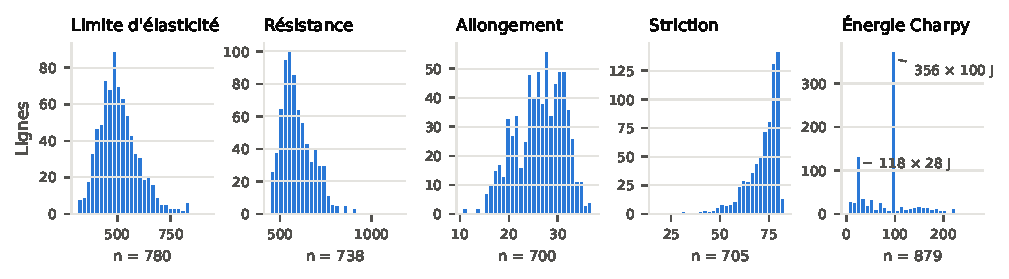
\includegraphics[width=\linewidth]{cibles}
  \caption{Distribution des cinq grandeurs à prédire ($n$ : nombre de lignes où elle est
    mesurée).}
  \label{fig:cibles}
\end{figure}

\paragraph{Valeurs extrêmes.} La règle de l'IQR ne convient pas : 64\,\% des
températures entre passes valent exactement \SI{200}{\celsius}, et elle déclarerait
aberrantes toutes les autres. Nous avons donc examiné les valeurs extrêmes une à une.
Ce sont presque toujours des mesures réelles, que nous gardons :
\begin{itemize}
  \item des séries volontaires (10 soudures très riches en soufre et en phosphore) ;
  \item des soudures hors norme mais cohérentes (une soudure à 9\,\% de chrome a la plus
    forte résistance et le plus faible allongement) ;
  \item un effet de source (l'article le plus ancien, Wolst-1974, détient quatre valeurs
    extrêmes).
\end{itemize}

\outrouver{revue détaillée : \code{preprocessing/outlier_*.py}, conclusions dans
\code{context/columns.json} (champ \code{outliers}).}

\subsubsection{Relations entre variables}

\paragraph{Corrélations.} La figure~\ref{fig:correlations} donne la corrélation de
Spearman (sur les rangs, donc peu sensible aux valeurs extrêmes) entre entrées et
grandeurs à prédire. Elle indique un lien, pas une cause.
\begin{itemize}
  \item Les éléments d'alliage (Cr, Mo, V, Nb) vont avec plus de résistance et moins de
    ductilité.
  \item Les réglages de soudage (courant, tension, énergie) et les impuretés (S, P) vont
    avec moins de striction.
  \item Le Charpy n'est fortement lié à aucune entrée de composition ou de soudage ; sa
    variable la plus liée est la température d'essai ($r = 0{,}46$).
\end{itemize}

\begin{figure}[!htbp]
  \centering
  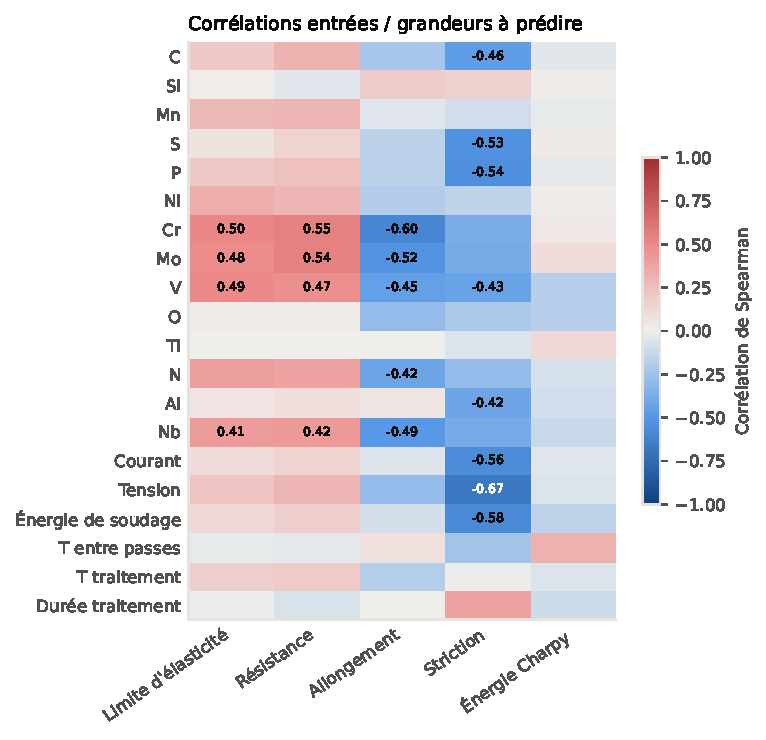
\includegraphics[width=0.62\linewidth]{correlations}
  \caption{Corrélation de Spearman entre entrées numériques et grandeurs à prédire. Les
    valeurs $|r| \geq 0{,}4$ sont écrites.}
  \label{fig:correlations}
\end{figure}

\paragraph{Analyse en composantes principales (ACP).} Appliquée aux 995 métaux distincts
(un métal testé plusieurs fois compte une fois), après imputation par la médiane et
standardisation (figure~\ref{fig:acp}) :
\begin{itemize}
  \item \textbf{les entrées ne sont pas redondantes} : deux axes n'expliquent que 38\,\%
    de la variance ; nous les gardons toutes ;
  \item \textbf{l'axe 1 (21\,\%) sépare aciers alliés et ordinaires} : les soudures
    riches en Cr, Mo, V, N et Nb sont presque toujours traitées thermiquement (94\,\% de
    celles à plus de 1\,\% de chrome), donc ces variables varient ensemble. On ne pourra
    pas distinguer l'effet des alliages de celui du traitement ;
  \item \textbf{l'axe 2 (17\,\%) correspond à la chaleur apportée par le soudage} : il
    sépare l'arc submergé (\SI{640}{\ampere} médian) de l'arc manuel (\SI{170}{\ampere}).
    Courant, tension et énergie de soudage varient ensemble, car l'énergie se calcule à
    partir des deux autres et de la vitesse : leurs effets ne pourront pas être séparés.
    Les recommandations porteront sur l'énergie, toujours renseignée et qui intègre la
    vitesse.
\end{itemize}
Ces résultats restent les mêmes avec d'autres méthodes d'imputation. Les modèles devront
couvrir des familles de soudures très différentes.

\begin{figure}[!htbp]
  \centering
  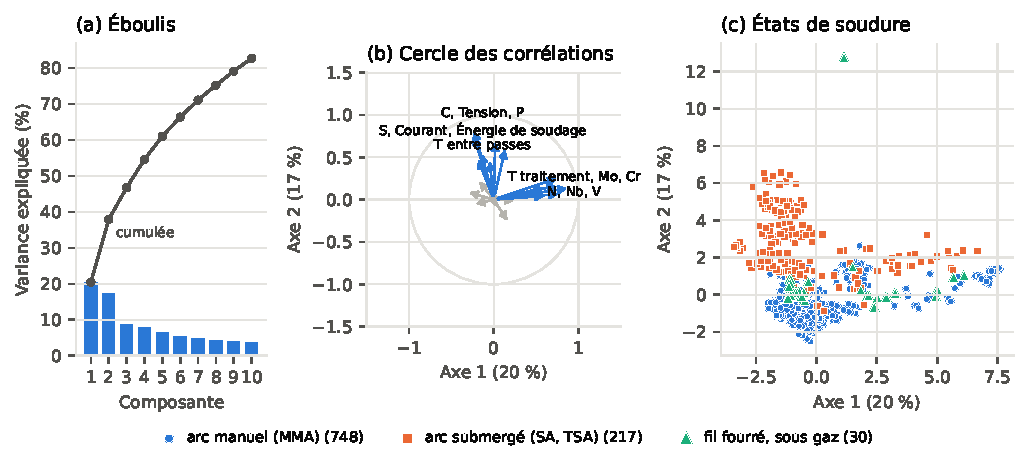
\includegraphics[width=\linewidth]{acp}
  \caption{ACP des entrées numériques : (a) variance expliquée par composante,
    (b) cercle des corrélations (flèches bleues : variables bien représentées), (c)
    projection des 995 métaux, par famille de procédé.}
  \label{fig:acp}
\end{figure}

\outrouver{notebook, « Analyse descriptive » (figures enregistrées dans
\code{report/figures/}) et « Énergie de soudage, courant et tension ».}

\afaire{\item Ajouter au notebook la comparaison des méthodes d'imputation avant l'ACP
    (médiane, plus proches voisins, imputation itérative).
  \item À décider en équipe : le traitement à \SI{250}{\celsius} / \SI{14}{\hour}
    (333 lignes, surtout de traction) est-il un simple dégazage équivalent à « brut » ?
  \item Recopier les résultats de traction sur les lignes Charpy du même état, utile
    seulement si la qualité combine résistance et ténacité.}

\subsection{Pré-traitement}\label{sec:preprocessing}

Trois problèmes sont traités dans l'ordre : valeurs manquantes, valeurs non numériques,
écarts d'échelle. Chaque étape est un script de \code{preprocessing/}, expliqué dans le
notebook ; le fichier d'origine n'est jamais modifié.

\subsubsection{Gestion des valeurs manquantes}\label{sec:prep-manquantes}

\paragraph{Colonnes écartées.} Les sorties absentes d'au moins trois quarts des lignes
(dureté, FATT, microstructure) et les entrées vides au moins une fois sur deux et
secondaires (Cu, Co, W, B, Sn, As, Sb, surtout à l'état de traces). Ni, Cr, Mo et Nb,
également vides à plus de 50\,\%, sont gardés : ce sont les principaux éléments
d'alliage (figure~\ref{fig:manquants}).

\begin{figure}[!htbp]
  \centering
  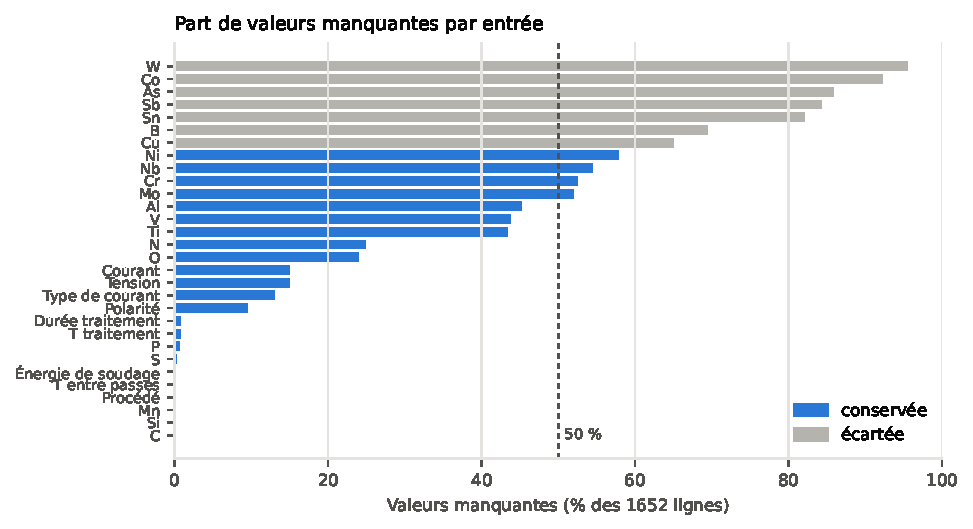
\includegraphics[width=0.82\linewidth]{manquants}
  \caption{Part de valeurs manquantes pour chacune des 30 entrées. En gris, les entrées
    écartées.}
  \label{fig:manquants}
\end{figure}

\paragraph{Valeurs déduites.}
\begin{itemize}
  \item \emph{Type de courant} (manquant sur 215 lignes) : une polarité \code{+} ou
    \code{-} implique le courant continu, \code{0} le courant alternatif ; 59 lignes
    complétées.
  \item \emph{Traitement thermique} (manquant sur 13 lignes notées « traitées » d'un
    même article) : nous supposons le traitement des autres soudures de l'article,
    \SI{600}{\celsius} pendant \SI{0,75}{\hour}.
\end{itemize}

\paragraph{Indicateurs de traitement.} Lue comme une quantité, la température ferait de
\SI{250}{\celsius} un demi-revenu. Or le traitement à \SI{250}{\celsius} /
\SI{14}{\hour} (333 lignes) est probablement un dégazage qui modifie peu le métal, alors
qu'un revenu entre 550 et \SI{750}{\celsius} le transforme. Deux entrées 0/1, « soudure
brute » (610 lignes) et « dégazage », permettent au modèle de traiter ces cas à part.

\paragraph{Valeurs complétées.} Les autres valeurs manquantes des entrées sont remplacées
par la médiane, avec pour chaque colonne un \emph{indicateur} 0/1 « valeur manquante » :
l'absence renseigne sur l'article (section~\ref{sec:exploration}). Cet indicateur décrit
la collecte des données, pas le métal (« nickel manquant » ne veut pas dire « sans
nickel ») : il ne servira pas aux recommandations. Les résultats d'essais ne sont jamais
complétés.

\outrouver{colonnes écartées : liste \code{DROPPED} dans \code{build_model_table.py}
(étape 5) ; type de courant : \code{categorical_clean.py} (étape 4) ; traitement inconnu :
\code{heat_treatment.py} (étape 4b) ; indicateurs de traitement : \code{INDICATORS} dans
\code{ml_dataset.py} ; imputation : \code{make_preprocessor} (étape 6).}

\afaire{\item Vérifier dans l'article Gar\&K-1975 le traitement des soudures de
    \SI{25}{\milli\metre} (supposé identique à celui des \SI{12}{\milli\metre}).
  \item Comparer l'imputation par la médiane à une imputation qui tient compte des autres
    colonnes (plus proches voisins, imputation itérative).}

\subsubsection{Gestion des variables non numériques}

\paragraph{Nombres écrits en texte.} Voir le tableau~\ref{tab:decodage}.

\begin{table}[!htbp]
  \centering\small
  \begin{tabularx}{\linewidth}{@{}l l r Y@{}}
    \toprule
    \textbf{Codage} & \textbf{Col.} & \textbf{Valeurs} & \textbf{Règle et justification} \\
    \midrule
    \code{<x} (limite de détection) & 14 col. & 1576 & $x$. La vraie valeur est entre 0
                                                       et $x$. Autre choix possible : $x/2$. \\
    V \code{<5}                     & 9       & 9    & 0,0005\,\%. C'est 5\,ppm : ailleurs,
                                                       V ne dépasse jamais 0,32\,\%. \\
    Ti, Al \code{<0.01}             & 14, 16  & 32   & \SI{100}{ppm}. C'est 0,01\,\% :
                                                       0,01\,ppm serait irréaliste. \\
    \code{67tot33res} (azote)       & 15      & 59   & 67. On garde l'azote total, comme
                                                       sur les autres lignes. \\
    \code{150-200} (entre passes)   & 27      & 38   & \SI{175}{\celsius}, le milieu de
                                                       l'intervalle. \\
    \bottomrule
  \end{tabularx}
  \caption{Conversion des nombres écrits sous forme de texte.}
  \label{tab:decodage}
\end{table}

\paragraph{Variables catégorielles.} Type de courant, polarité et procédé sont convertis
par \emph{encodage one-hot} (une colonne 0/1 par catégorie) : étant nominales, un
encodage ordinal (0, 1, 2\ldots) leur imposerait un ordre qui n'existe pas. Les 10 codes de procédé sont
d'abord regroupés en 5 familles selon la protection du métal fondu (enrobage, flux en
poudre, fil fourré ou gaz), principale différence entre procédés à l'arc
(tableau~\ref{tab:procedes}). Cela fusionne les synonymes (ShMA et MMA) et les codes de 4
à 7 lignes, trop rares pour être appris ; la famille sous gaz reste hétérogène.

\begin{table}[!htbp]
  \centering\small
  \begin{tabular}{@{}l l r@{}}
    \toprule
    \textbf{Famille} & \textbf{Codes d'origine (lignes)} & \textbf{Lignes} \\
    \midrule
    MMA (arc manuel, électrode enrobée) & MMA (1140), ShMA (40, même procédé) & 1180 \\
    SA (arc submergé sous flux)         & SA (261), NGSAW (18), SAA (4)       & 283 \\
    TSA (arc submergé, deux fils)       & TSA (87)                            & 87 \\
    FCA (fil fourré)                    & FCA (87)                            & 87 \\
    GSA (arc sous protection gazeuse)   & NGGMA (7), GMAA (4), GTAA (4)       & 15 \\
    \bottomrule
  \end{tabular}
  \caption{Regroupement des procédés de soudage en cinq familles.}
  \label{tab:procedes}
\end{table}

\outrouver{\code{decensor.py} (étape 1), \code{nitrogen_total.py} (étape 2),
\code{interpass_range.py} (étape 3), \code{categorical_clean.py} (étape 4) ; encodage :
\code{make_preprocessor} dans \code{ml_dataset.py} (étape 6).}

\afaire{\item Tests de sensibilité : \code{<x} $\rightarrow x$ ou $x/2$ ; azote total ou
    total + résiduel.}

\subsubsection{Mise à l'échelle}

Le carbone varie entre 0,03 et 0,18\,\%, le courant entre 115 et \SI{900}{\ampere}. Nous
\emph{standardisons} toutes les variables numériques (moyenne 0, écart-type 1) :
\begin{itemize}
  \item \textbf{nécessaire} pour les modèles sensibles à l'échelle : Ridge, Lasso, ACP,
    PLS, plus proches voisins, SVR, réseaux de neurones ;
  \item \textbf{sans effet} sur les prédictions des autres : régression linéaire simple,
    arbres et forêts (un arbre coupe au même endroit quelle que soit l'unité).
\end{itemize}
Tous les modèles reçoivent ainsi la même préparation. Limites : la standardisation est
sensible aux valeurs extrêmes et ne corrige pas l'asymétrie ; une mise à l'échelle
robuste ou une transformation logarithmique seront comparées.

\paragraph{Éviter la fuite d'information.} Imputation, encodage et standardisation
utilisent des statistiques des données (médiane, moyenne\ldots). Calculées sur toute la
base, elles feraient profiter l'entraînement des données de test et rendraient les
résultats trop optimistes. Un \code{Pipeline} scikit-learn les recalcule sur les seules
données d'entraînement, à chaque étape de l'évaluation.

\outrouver{\code{make_preprocessor} dans \code{preprocessing/ml_dataset.py} (étape 6).}

\afaire{\item Transformations des variables asymétriques (log1p, mise à l'échelle robuste).
  \item Vérifier la température Charpy de \SI{188}{\celsius} (\code{Ditt-0.5rch2}).}

\section{Modélisation}\label{sec:methodes}

\subsection{Protocole d'évaluation}\label{sec:protocole}

Tous les modèles suivent le même protocole, pour être comparables.

\subsubsection{Variables à prédire}\label{sec:qualite}

\paragraph{Pourquoi ces grandeurs.} La base ne dit pas si une soudure est « bonne ».
Nous mesurons sa qualité par les propriétés que vérifient les normes de soudage : la
\emph{résistance} et la \emph{ductilité} (essai de traction), et la \emph{ténacité},
résistance aux chocs (essai Charpy). L'absence de défauts ou la tenue en fatigue ne sont
pas dans la base.

\paragraph{Ce que les données en disent.}
\begin{itemize}
  \item Limite d'élasticité et résistance à la traction sont presque redondantes
    (corrélation 0,93 sur 714 lignes).
  \item La résistance s'oppose à la ductilité (corrélations de $-0{,}57$ à $-0{,}78$) :
    une bonne soudure est un compromis.
  \item Les lignes Charpy sont de deux types : 405 énergies mesurées, 474 fixées à
    \SI{100}{\joule} ou \SI{28}{\joule} (section~\ref{sec:exploration}).
\end{itemize}

\begin{table}[!htbp]
  \centering\small
  \begin{tabular}{@{}l l c r r@{}}
    \toprule
    \textbf{Qualité} & \textbf{Grandeur} & \textbf{Unité} & \textbf{Lignes} & \textbf{Articles} \\
    \midrule
    Résistance & \textbf{limite d'élasticité} & \si{\mega\pascal} & 780 & 42 \\
               & résistance à la traction     & \si{\mega\pascal} & 738 & 41 \\
    Ductilité  & \textbf{allongement}         & \%                & 700 & 36 \\
               & striction                    & \%                & 705 & 34 \\
    Ténacité   & \textbf{énergie Charpy}      & \si{\joule}       & 879 & 26 \\
    \bottomrule
  \end{tabular}
  \caption{Grandeurs mesurant la qualité. En gras, les trois cibles principales.}
  \label{tab:cibles}
\end{table}

\paragraph{Stratégie.}
\begin{enumerate}
  \item \textbf{Prédire chaque propriété} : une cible principale par qualité (en gras,
    tableau~\ref{tab:cibles}), chacune avec son modèle de régression, entraîné sur les
    lignes où elle est mesurée. Pour le Charpy, la température d'essai est une entrée ;
    c'est une condition de mesure, pas un réglage : les recommandations seront données
    pour une température d'essai fixée.
  \item \textbf{Juger la qualité} : la soudure est bonne si chaque valeur prédite dépasse
    son seuil.
\end{enumerate}
Un modèle direct « bonne / mauvaise » serait moins adapté : les seuils dépendent de
l'usage, un oui/non perd de l'information (avec un seuil de \SI{47}{\joule},
\SI{46}{\joule} et \SI{10}{\joule} seraient tous deux « mauvais »), et résistance et
ténacité sont rarement mesurées sur la même ligne.

Ce choix exclut les modèles de classification, pas les familles de modèles (arbres,
forêts, plus proches voisins existent en régression). Son coût : la régression ne se
concentre pas sur les erreurs proches du seuil. Une classification est donc testée en
complément sur le Charpy, seule propriété avec un seuil commun à tous les aciers
(\SI{27}{\joule} ou \SI{47}{\joule}) ; le seuil de résistance dépend de la classe d'acier
(section~\ref{sec:modeles}).

\outrouver{\code{TARGETS} et \code{get_xy} dans \code{preprocessing/ml_dataset.py} ;
notebook, étape 6 et « Analyse descriptive › Liens entre les grandeurs à prédire ».}

\afaire{\item Valider en équipe les trois cibles principales.
  \item Trouver les seuils de « bonne soudure » et leurs sources (normes ISO 2560,
    ISO 15614-1, AWS A5.1 à vérifier ; seuils Charpy usuels de \SI{27}{\joule} ou
    \SI{47}{\joule} à une température donnée).}

\subsubsection{Validation croisée}

Un modèle est jugé sur des données qu'il n'a pas vues : la \emph{validation croisée}
découpe les données en 5 parts, entraîne sur 4, teste sur la cinquième, cinq fois, puis
moyenne les scores. Les lignes d'un même cordon ou d'un même article étant très proches,
un découpage au hasard serait trop optimiste. Les lignes sont donc regroupées
\textbf{par article} (\code{GroupKFold}) : le score mesure la capacité à prédire les
soudures d'une étude inconnue.

\outrouver{fonction \code{weld_source} dans \code{preprocessing/ml_dataset.py} ;
vérification de l'absence de fuite : notebook, étape 6.}

\afaire{\item Validation croisée imbriquée : un niveau extérieur (par article) pour mesurer
    la performance, un niveau intérieur (par article) pour régler les hyperparamètres.
  \item Ne pas utiliser l'erreur OOB des forêts : elle ignore les articles et serait trop
    optimiste.}

\subsubsection{Mesures d'erreur}

\afaire{\item Justifier les mesures : RMSE et MAE, dans l'unité de la cible
    (\si{\mega\pascal}, \%, \si{\joule}), et $R^2$ ; moyenne $\pm$ écart-type sur les plis.
  \item Choix final par la règle de l'écart-type (cours 2) : parmi les modèles presque
    aussi bons que le meilleur, garder le plus simple.
  \item Coder le protocole commun (modèle + cible $\rightarrow$ scores), à faire en
    premier --- \textbf{Salomé (proposé)}.}

\subsection{Entraînement et évaluation des modèles}\label{sec:modeles}

Chaque famille de modèles est appliquée aux trois cibles principales.

\subsubsection{Modèles de référence et modèles linéaires}

\afaire{\item Référence : prédire la moyenne (tout modèle doit faire mieux).
  \item Régression linéaire, sélection de variables pas à pas, Ridge, Lasso ; lecture des
    coefficients --- \textbf{Salomé (proposé)}.}

\subsubsection{Réduction de dimension}

\afaire{\item Régression sur les composantes de l'ACP et PLS ; nombre de composantes réglé
    par validation croisée.
  \item Charpy : modéliser les deux types de lignes ensemble ou séparément ? Tester les
    deux --- \textbf{?}}

\subsubsection{Arbres et méthodes d'ensemble}

\afaire{\item Arbre CART, bagging, forêt aléatoire, extra-trees ; hyperparamètres
    (profondeur, taille minimale des feuilles, nombre de variables tirées).
  \item Importance des variables par permutation ; attention aux variables corrélées
    (Cr, Mo, traitement), dont l'importance est surestimée --- \textbf{?}
  \item Classification complémentaire « Charpy $\geq$ \SI{47}{\joule} à la température
    d'essai ? » : comparer un arbre ou une forêt de classification au même modèle en
    régression suivi du seuil, sur les mêmes plis.
    \begin{itemize}
      \item Seulement les 405 énergies mesurées (13 articles) : sur les lignes fixées,
        l'étiquette est imposée par la convention (\SI{100}{\joule} toujours « bonne »,
        \SI{28}{\joule} toujours « mauvaise »).
      \item Classes déséquilibrées (69\,\% de « bonnes » à \SI{47}{\joule}, 84\,\% à
        \SI{27}{\joule}) : précision équilibrée, F1, matrice de confusion.
      \item Piste facultative : classes de résistance de la norme des électrodes
        (ISO 2560, seuils à vérifier) pour la traction.
    \end{itemize}}

\subsubsection{Apprentissage semi-supervisé}

\afaire{\item Bibliographie et au moins une méthode (auto-apprentissage, co-régression
    COREG) exploitant les lignes où la cible n'est pas mesurée ; justifier son
    intérêt --- \textbf{?}}

\subsection{Conclusion de la modélisation}\label{sec:resultats}

\afaire{\item Tableau comparatif des modèles par cible (moyenne $\pm$ écart-type sur les plis).
  \item Figures prédit / réel.
  \item Poids des indicateurs « valeur manquante » (section~\ref{sec:prep-manquantes}) :
    comparer avec et sans.
  \item Modèle retenu pour chaque cible et limites (peu d'articles, extrapolation).
  \item Chacun présente sa famille de modèles aux autres avant le partiel.}

% Gabarit de tableau à remplir
% \begin{table}[!htbp]
%   \centering\small
%   \begin{tabular}{@{}lccc@{}}
%     \toprule
%     \textbf{Modèle} & \textbf{RMSE (MPa)} & \textbf{MAE (MPa)} & $\boldsymbol{R^2}$ \\
%     \midrule
%     Ridge  & & & \\
%     \bottomrule
%   \end{tabular}
%   \caption{Limite d'élasticité, validation croisée groupée par article.}
% \end{table}

\section{Conclusion et recommandations}\label{sec:conclusion}

\afaire{\item Approche la plus appropriée pour prédire la qualité de soudure.
  \item Recommandations pour une bonne soudure (variables influentes, plages favorables),
    avec leurs limites : corrélations issues de la littérature, pas de causalité.}


\end{document}
